\section{Gravity waves}

Gravity waves test taken from Weller and Shahrokhi.

\begin{itemize}
\item Reproduced result for BTF from W\&S
\item Vertical mixing at ground in lee of orography seen in results for snapCol and snap meshes.  This occurs in the lowest two rows of the mesh: lower layer $\theta$ is warmer, next layer above is cooler.  Feature is visible after t=3600s (Figure~\ref{fig:gw:mixing-3600s}), becomes more pronounced by t=18000s (Figure~\ref{fig:gw:mixing-18000s}).
\end{itemize}

\subsection{TODO: investigate vertical mixing}
Suspect mixing is computational mode of Lorenz vertical staggering but need to confirm:
\begin{itemize}
\item plot UfDiff (as a vector field?) to see velocity anomalies
\item plot $\theta$ field, see if we would expect vertical motion in lowest two mesh rows
\item if we expect $w \neq 0$ but no motion is present in simulation, we have found computational mode
\end{itemize}

To see if the computational mode is present in >1 test case, try:
\begin{itemize}
\item halving $\Delta z$ --- are 2 rows of cells still affected (suggests computational mode), or 4 rows (physical problem?)
\item increase mountain height (currently mountain top = 250m, $\Delta z$ = 300m)
\item change stability (zN in environmentalProperties)
\end{itemize}

\begin{figure}
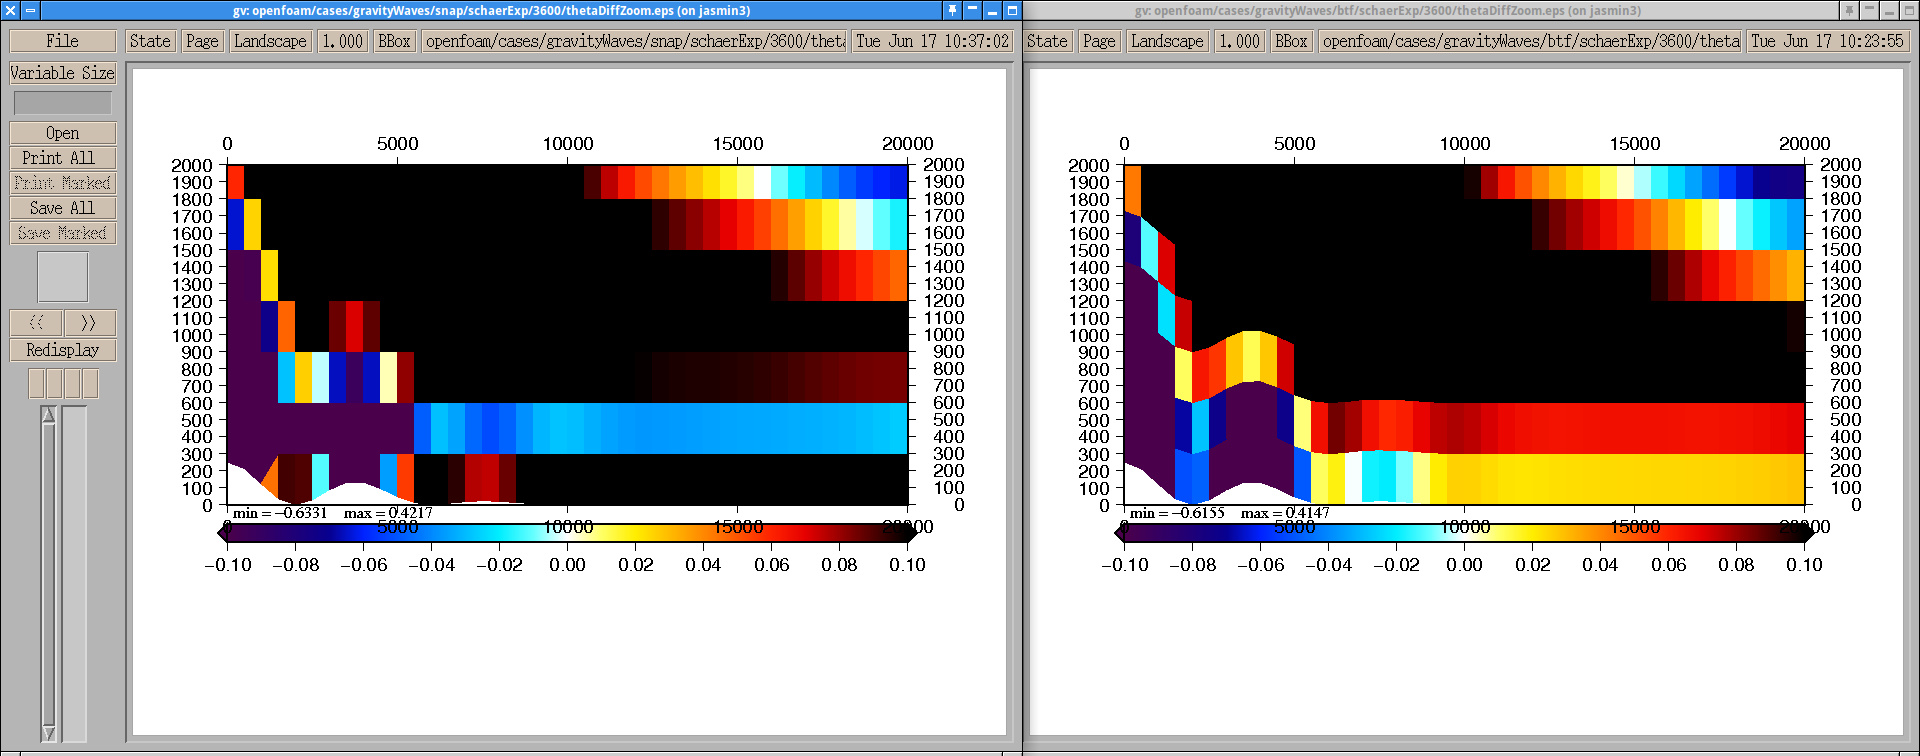
\includegraphics[width=\textwidth]{interim-results/gravityWavesBTFsnapMidZoom3600.png}
\caption{Vertical mixing after t=3600s, snap mesh left, BTF right}
\label{fig:gw:mixing-3600s}
\end{figure}

\begin{figure}
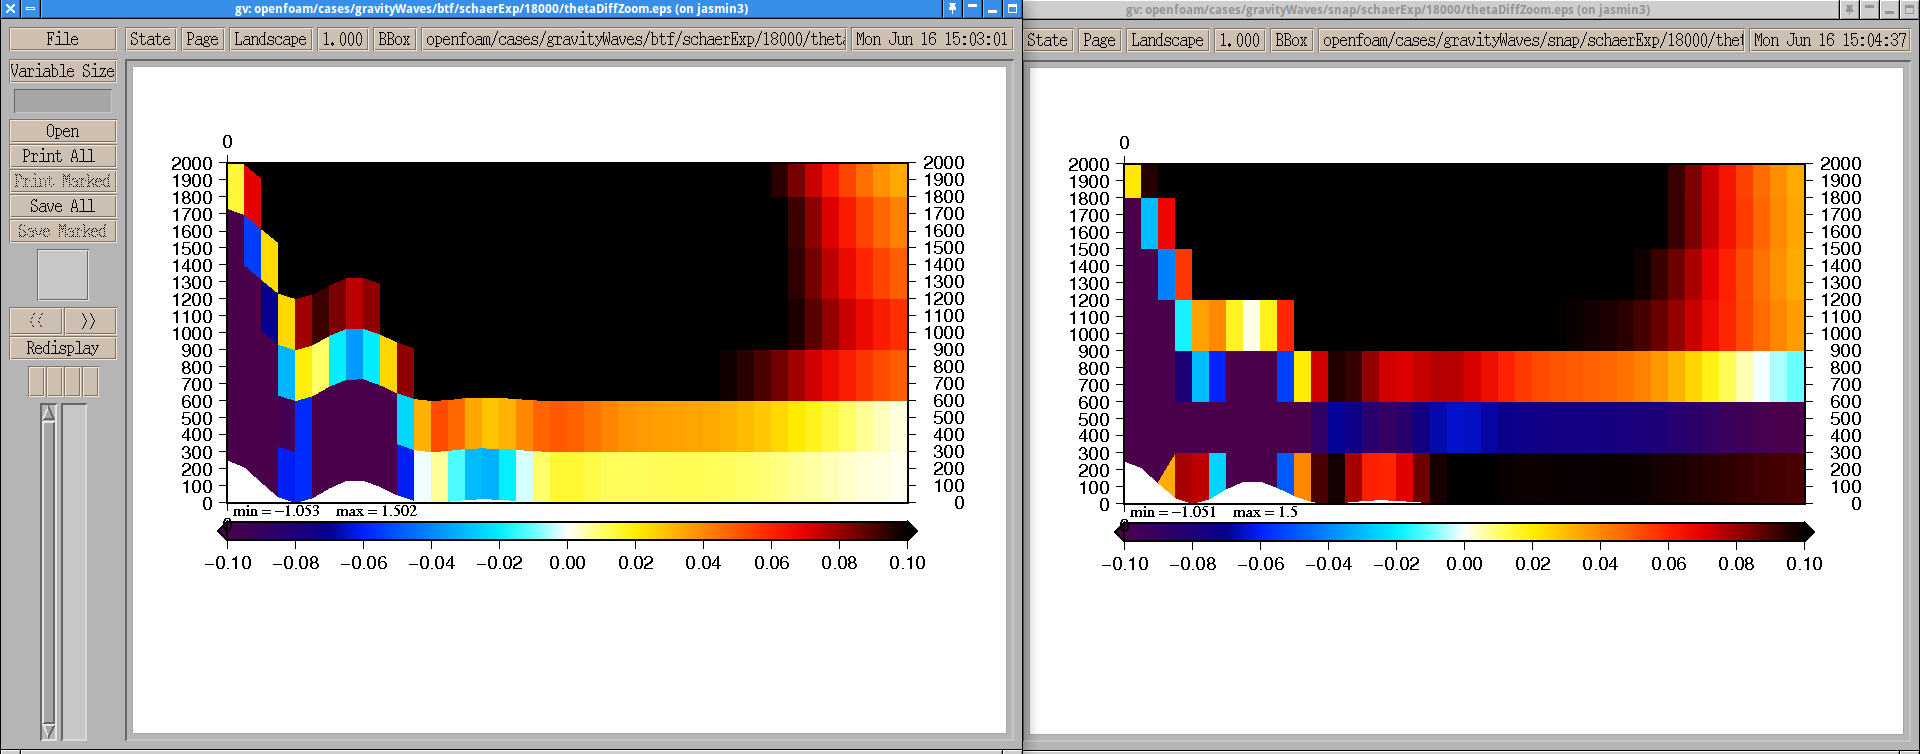
\includegraphics[width=\textwidth]{interim-results/gravityWavesBTFsnapMidZoom18000.png}
\caption{Vertical mixing after t=18000s.  Confusingly, snap mesh right, BTF left!}
\label{fig:gw:mixing-18000s}
\end{figure}
